%!TEX root = ../terrainbook.tex

\graphicspath{{visibility/}}

\chapter{Visibility queries on terrains}

\begin{figure}[ht]
  \centering
  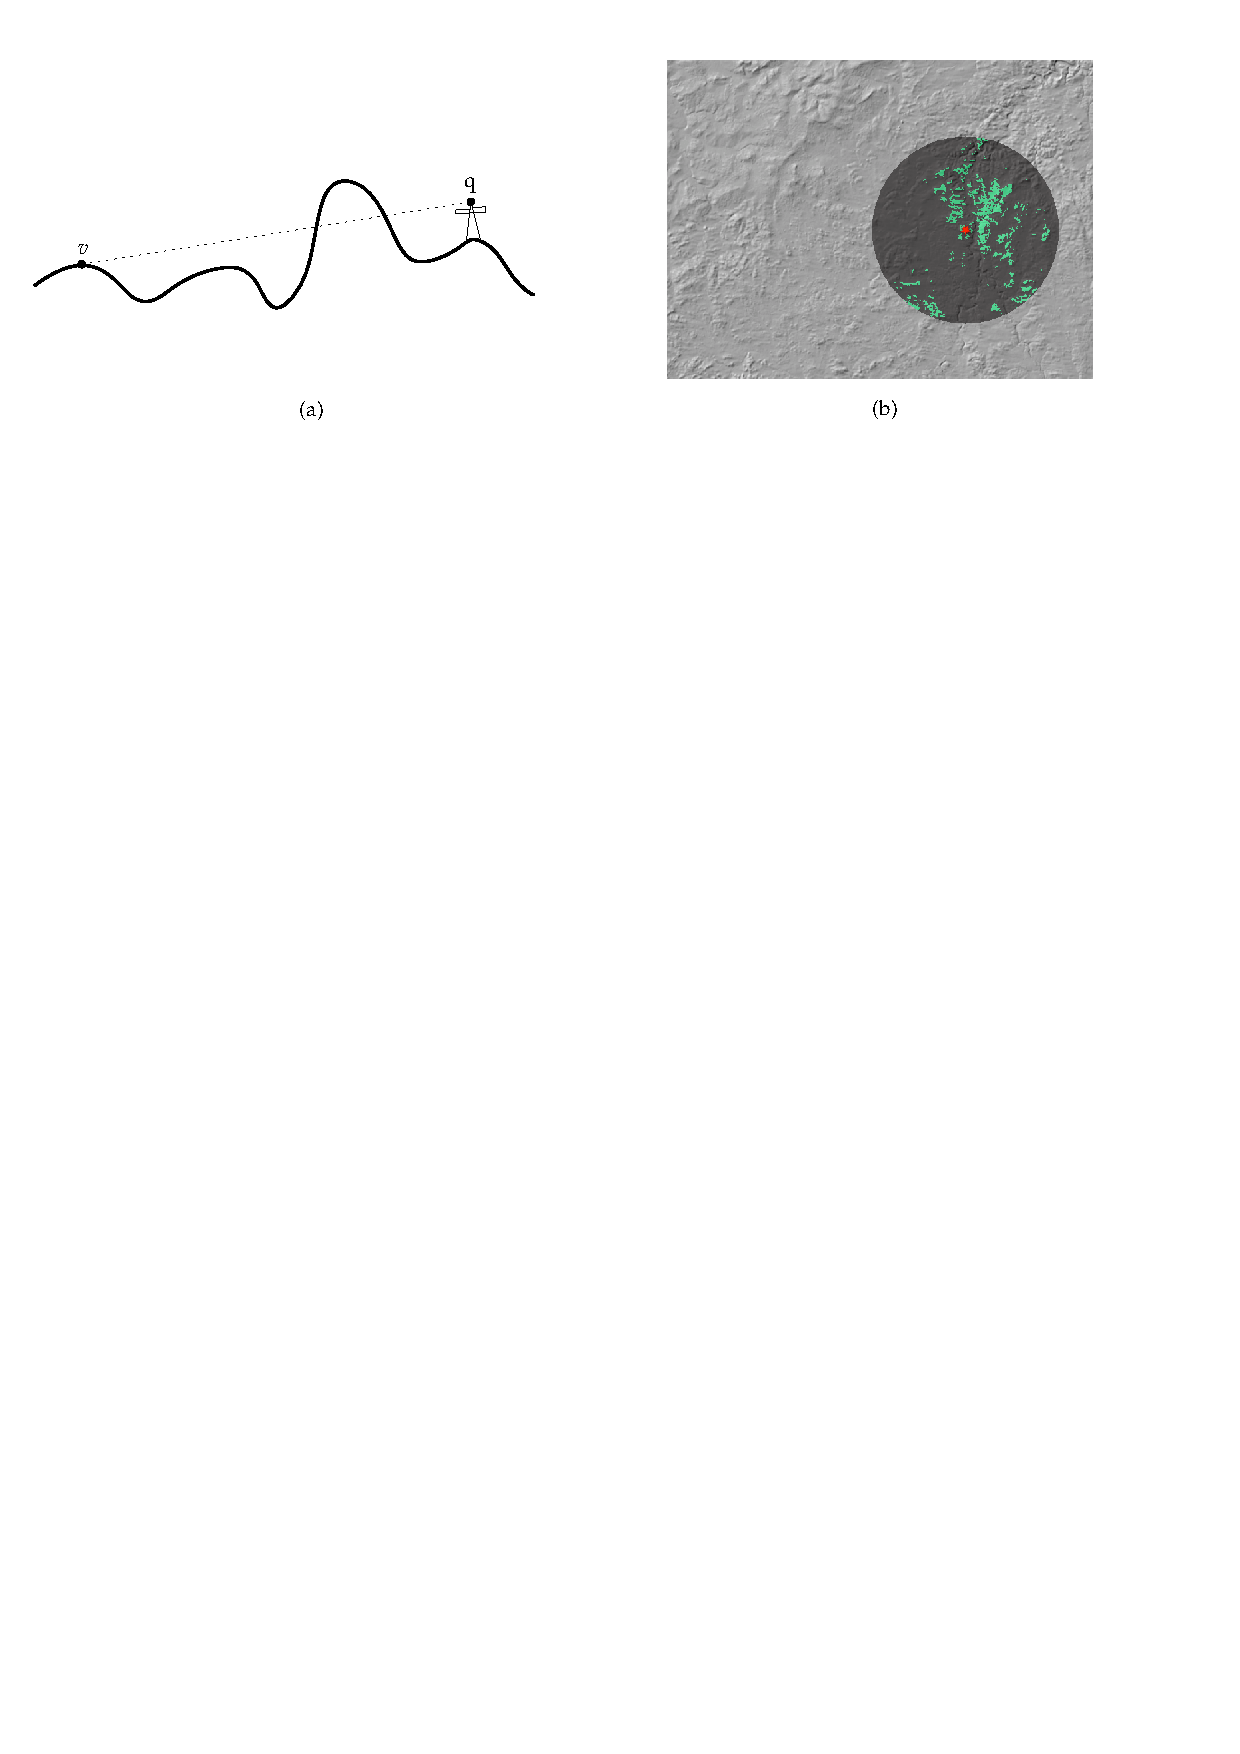
\includegraphics[width=\linewidth]{figs/overview_los_viewshed.pdf}
  \caption{\textbf{(a)} Line-of-sight between $v$ and $q$; $q$ is not visible. \textbf{(b)} The viewshed at the location marked with a red star (green = visible; maximum view distance (dark grey) is set to 15km).}
\label{fig:overview_los_viewshed}
\end{figure}

Several applications using terrains involve \emph{visibility queries}, \ie\ given a viewpoint, which part(s) of the surrounding terrain are visible.
Examples of such applications are many: optimal position of telecommunication towers, path planning for hiking (to ensure the nicest views), estimation of the view for scenic drives, estimation of visual damage when trees in a forest are cut, etc.
There are also several related problems.
One example is the estimation of shadows (position of the sun continually varies, also with seasons).
Shadows are important to accurately measure the photovoltaic potential, for determining solar envelopes, for assessing the value of real estate, and for estimating the thermal comfort, among other applications.

%

When referring to visibility problems, we address the following two fundamental problems:
\begin{description}
  \item[line-of-sight (LoS):] given a viewpoint $v$ and another point $q$, does $v$ sees $q$ (and vice-versa)?; or, in other words, does the segment $vq$ intersects the terrain? The result is either True or False.
  \item[viewshed:] given a viewpoint $v$, which part(s) of the surrounding terrain are visible? The result is a polygon (potentially disconnected) showing the locations and extent of what is visible from $v$. Usually the extent is limited to a certain ``horizon'', or radius of visibility. If the terrain is formed of different objects (\eg\ buildings), an object is either visible or not (simple case), or parts of objects can be visible (more complex).
\end{description}
Observe that for both problems, the viewpoint can either be directly on the terrain (at relative elevation 0m) or at a given height (2m for a human, or 30m for a telecommunication tower).

%

We discuss in this lesson the general problem of visibility as defined in computer graphics, and then discuss how terrains, being 2.5D surfaces, simplify the problem.
We discuss how to solve these problems for both TINs and grids.
% , and then we briefly explain how point clouds can be directly used for such queries.




%%%%%%%%%%%%%%%%%%%%
%
\section{Rendering + ray casting}

Rendering is the process of generating images from 2D or 3D scenes.
Without going into details, as shown in Figure~\ref{fig:Ray_trace_diagram}, it involves projecting the (3D) objects in a scene to an image (say 800x800 pixels) and assigning one colour to each pixel.
\begin{figure}
  \centering
  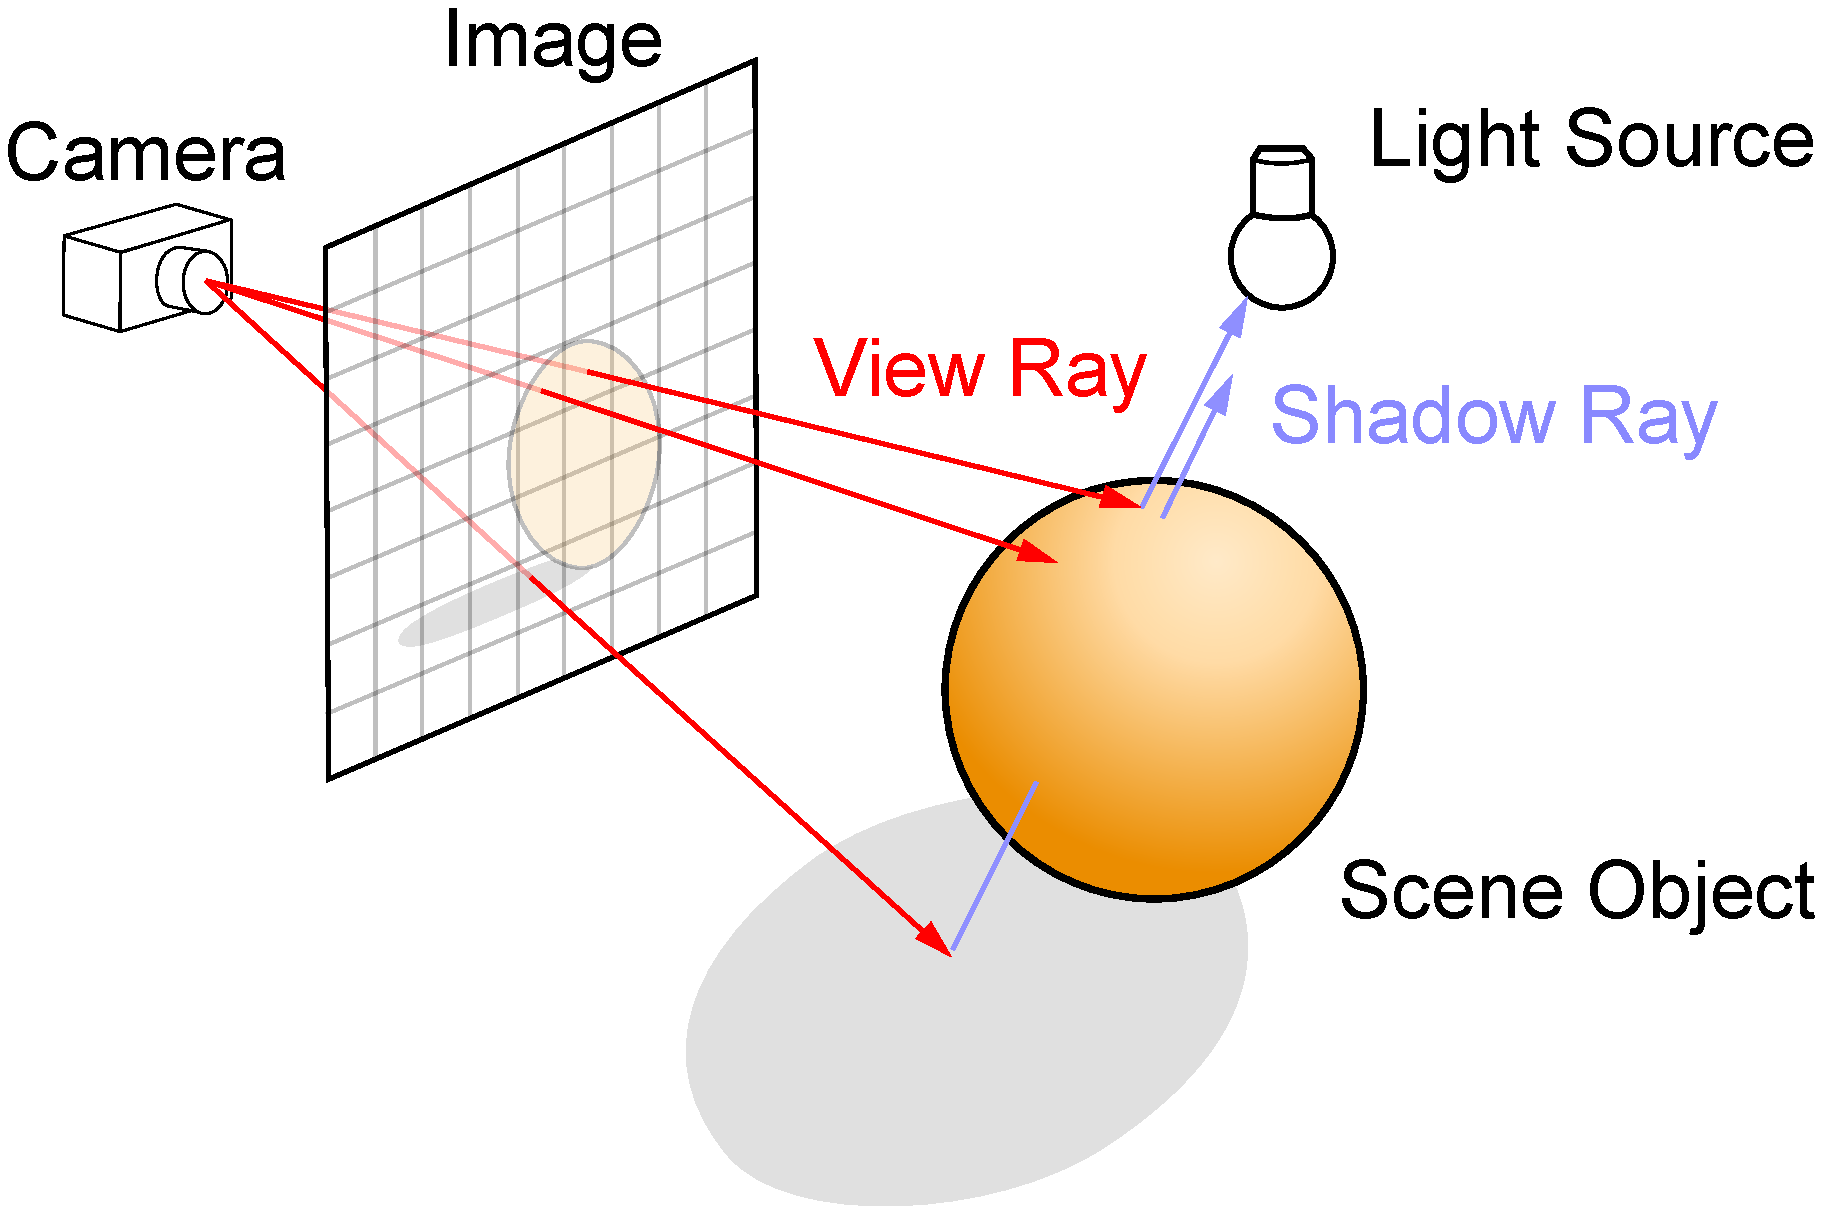
\includegraphics[width=0.6\linewidth]{figs/Ray_trace_diagram.pdf}
  \caption{Ray tracing builds the image pixel by pixel by extending rays into the scene. Figure from \url{https://commons.wikimedia.org/wiki/File:Ray_trace_diagram.svg}.}
\label{fig:Ray_trace_diagram}
\end{figure}
The colour of a pixel is that of the closest object, but to obtain photorealistic images, lighting, shading, and other physics-based functions are often applied (this goes beyond the scope of this course!).

Ray casting is used for each pixel: a ray is defined between the viewpoint $p$ and the centre of the pixel, and the closest object in the scene must be found.
The main issue involves finding that closest object, and especially discard the other objects lying behind it.


%%
\begin{link-box}
\textbf{Parts of the following chapter.} It summarises different methods to determine which surfaces are visible, for the generic cases of objects in 3D space.
Read only the following sections: 18.0, 18.1, 18.2, and 18.4.
\\
\bibentry{Salomon11}\\
\textbf{PDF:} \url{https://doi.org/10.1007/978-0-85729-886-7_18}

\end{link-box}


%%%%%%%%%%%%%%%%%%%%
%
\section{For 2.5D terrains, the problem is simpler}

% Simplifying the problem by sorting the triangles
The problem is simplified for terrains because a terrain is a 2.5D surface, and we can convert the problem to a 2D one.
Furthermore, we can exploit the connectivity and adjacency between the 2D cells forming a terrain to minimise the number of objects to test (for intersections and for determining who is in front of who).


%%%
%
\subsection{Visibility in TINs}

\begin{link-box}
\textbf{Parts of the following chapter.} 
Read from Section 1 to Section 3.1; it covers the simplest case for a LoS between 2 points on the surface.
\\
\bibentry{deBerg97}\\
\textbf{PDF:} \url{https://doi.org/10.1007/3-540-63818-0_4}
\end{link-box}


%%%
%
\subsection{Visibility in grids}

Solving visibility queries in grids is simpler than with triangles since the topology of the grid is implied (we have direct access to the neighbours of a given cell), and because grid cells are usually small we can assume that a grid cell is visible (or not) if its centre is visible (or not).
The same assumption is tricky for triangles, since these can be large; in practice it is often assumed that a triangle is visible if its 3 vertices are visible, but this varies per implementation.

%

We describe here how both LoS and viewshed queries can be implemented for grids; the same principles could be applied to TINs with minor modifications.


%%%
\paragraph{Line-of-sight.}
A LoS query, between a viewpoint $v$ and another point $q$, implies reconstructing the profile of the terrain along the vertical projection of $vq$ (let us call it $vq_{xy}$).
It then suffices to follow $vq$ and verify whether the elevation at any ($x,y$) location along the profile is higher than that of $vq$.
As shown in Figure~\ref{fig:los}, 
\begin{figure}
  \centering
  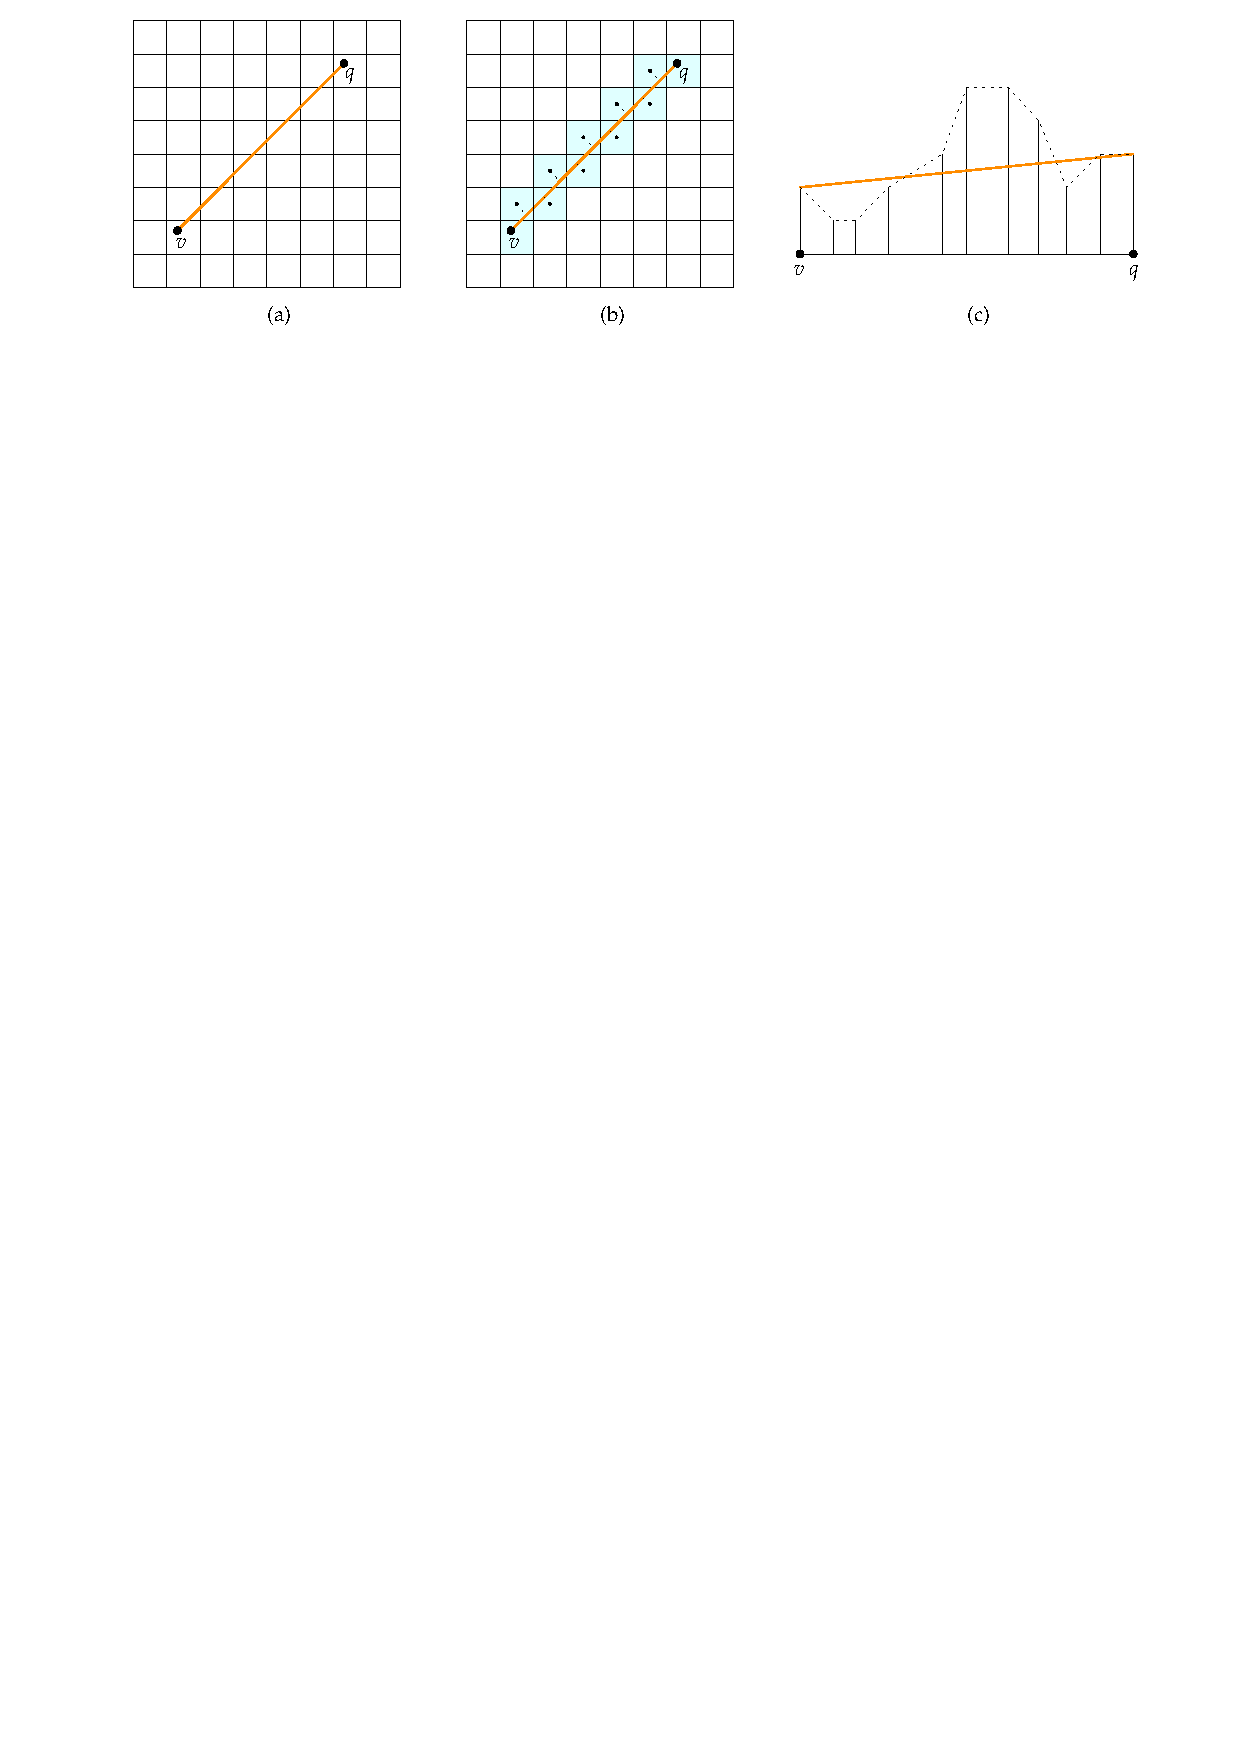
\includegraphics[width=\linewidth]{figs/los}
  \caption{Line-of-sight for between $v$ and $q$. Observe that along the profile, the points with elevation are not equally spaced.}
\label{fig:los}
\end{figure}
since the terrain is discretised into grid cells, there are 2 options to reconstruct the profile between $v$ and $q$:
\begin{enumerate}
  \item identify all the cells intersected by $vq_{xy}$, and assign the centre of each cell by projecting it to the terrain profile. This is what is done in Figure~\ref{fig:los}.
  \item consider the edges of the cells, collect all the edges that are intersected by $vq_{xy}$, and linearly interpolate the elevations. This is far more expensive to compute, and therefore less used in practice.
\end{enumerate}

The algorithm is thus as follows.
Start at $v$, and for each pixel $c$ encountered along $vq_{xy}$, verify whether the elevation value of $vq$ at that location is higher than the elevation of $c$.
If it is, then continue to the next pixel; if not, then there is an intersection and thus the visibility is False.
If the pixel containing $q$ is reached without detecting an intersection, then the visibility is True.


%%%
\paragraph{Viewshed.}
As shown in Figure~\ref{fig:viewshed},
\begin{figure}
  \centering
  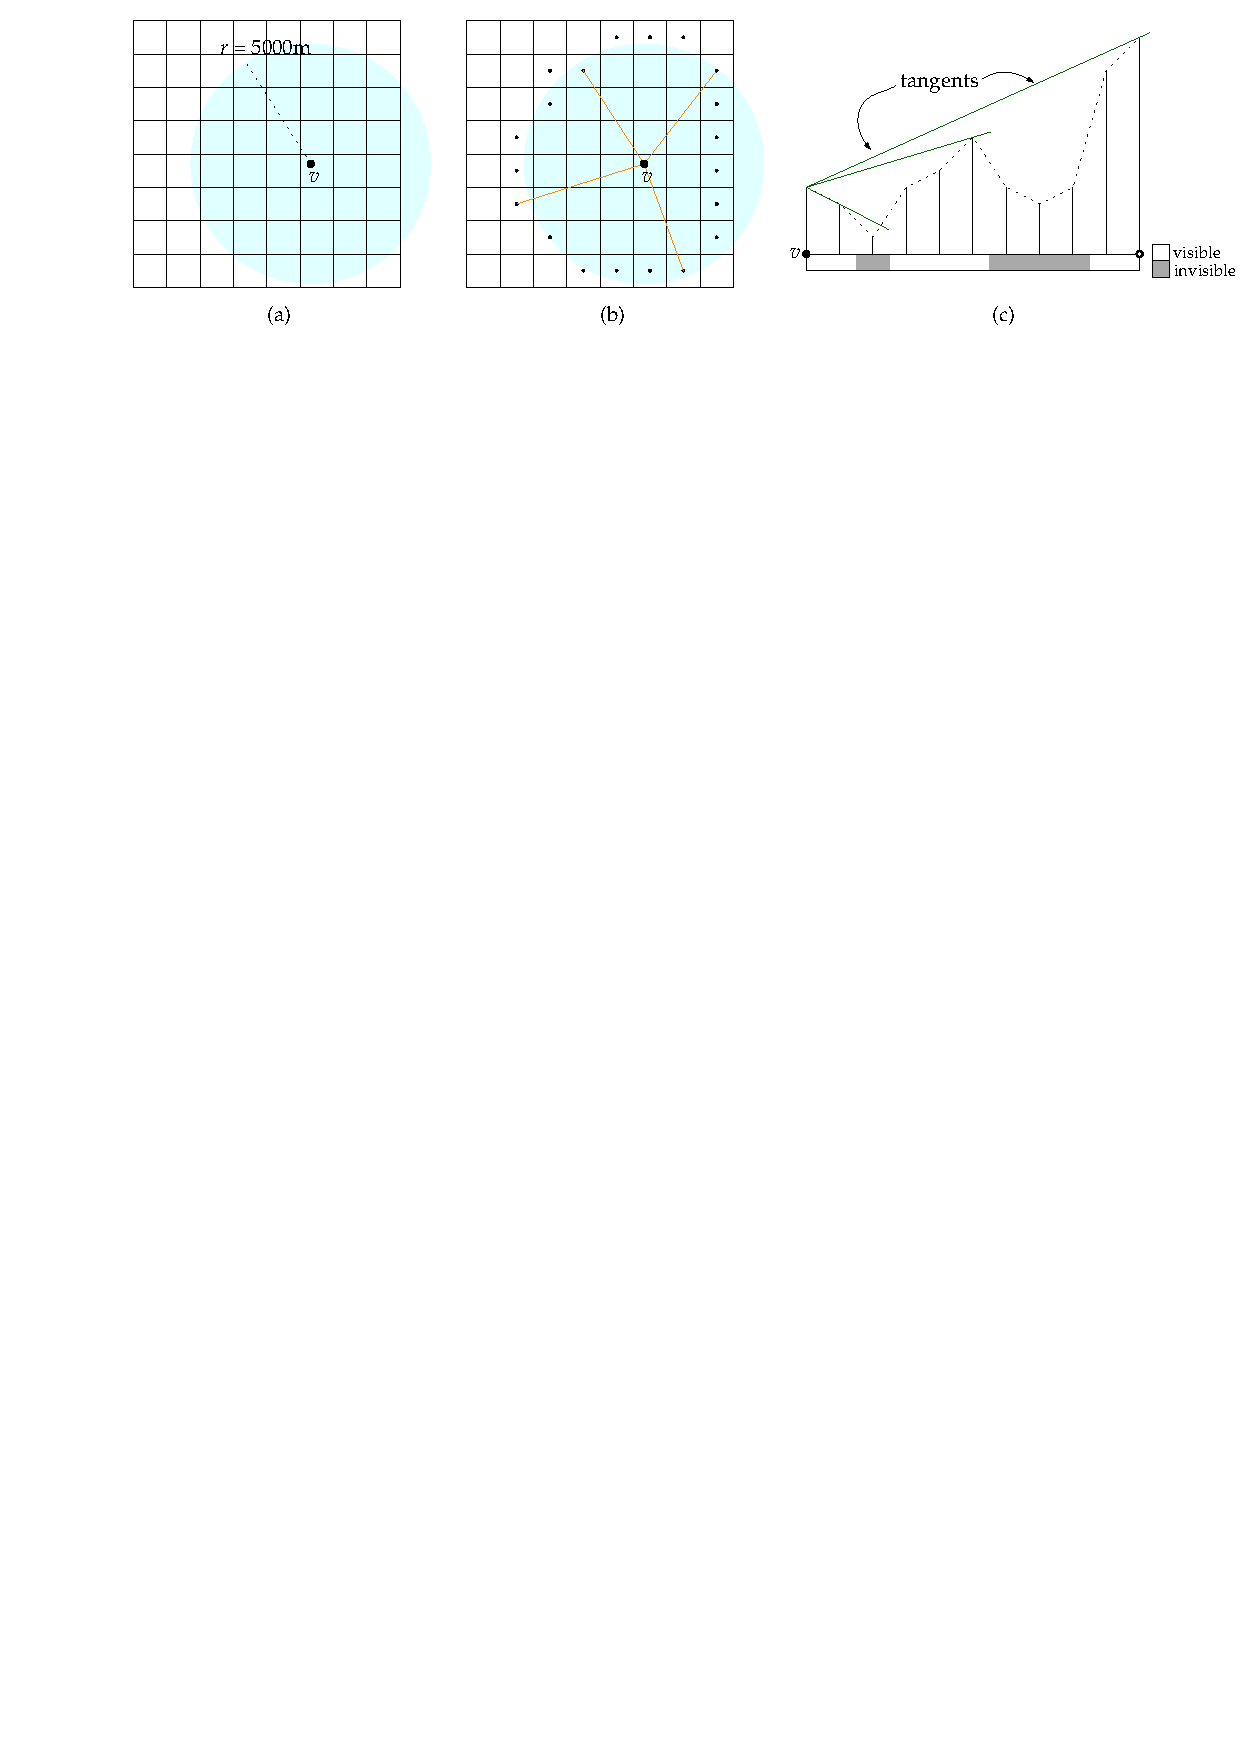
\includegraphics[width=\linewidth]{figs/viewshed}
  \caption{Viewshed for the point $v$; the blue circle is the radius of the horizon (5000km in this case).}
\label{fig:viewshed}
\end{figure}
computing the viewshed from a single viewpoint $v$ implies that the LoS between $v$ and the centre of each pixel in a given radius is tested. 
The result of a viewshed is a binary grid; in Figure~\ref{fig:overview_los_viewshed}b True/visible pixels are green, and False/invisible ones are dark grey.

%

While this brute-force approach will work, several redundant computations will be made, since several of the rays from $v$ will intersect the same grid cells.
Furthermore, depending on the resolution, the number of cells in a 5km radius (a reasonable value where humans can see) can become \emph{very} large.
As an example, with the AHN3 gridded version (50cm resolution), this means roughly 400M queries ($(\frac{5000 \times 2}{0.5})^2$).

%

One alternative solution is shown in Figure~\ref{fig:viewshed}b: it involves sampling the grid cells intersecting the border of the visible circle (obtaining several centres $q_i$), and computing the visibility of each of the cells along the line segment $vq_i$ as we `walk' from $v$.
Observe that, along $vq_i$, it is possible that a point far from $v$ is visible, while several closer points are not; Figure~\ref{fig:viewshed}c gives an example.

One solution involves using so-called \emph{tangents}.
The current tangent $t_{cur}$ is first initialised as a vector pointing downwards.
Then, starting at $v$, we walk along the ray $vq_i$, and for each cell intersected its elevation $z$ is compared to the elevation of $t_{cur}$ at that location.
If $z$ is lower, then the cell is invisible.
If $z$ is higher, then the cell is visible and $t_{cur}$ is updated with a new tangent using the current elevation.

Viewsheds with several viewpoints $v_i$ are also very useful, think for instance of obtaining the viewshed along a road.
This can be computed by sampling the road at every 50m and computing the viewsheds from each of the points. 
Each viewshed yields a binary grid, and it suffices to use a map algebra operator to combine the results into one grid (if one cell is visible from any viewpoint, then it is visible).


%%%%%%%%%%%%%%%%%%%%
%
% \section{Visibility in point clouds}
% TODO : ravi for 3D MAT overview? Just this solution perhaps? With filling voxels I guess?
% the lesson is already pretty long... so we decide what to do there.

% \begin{figure}
%   \centering
%   \begin{subfigure}[b]{0.3\linewidth}
%     \centering
%     
\includegraphics[width=\textwidth,page=1,trim=0 0 0 210, clip]{figs/mavis_diagrams.pdf}
%     \caption{}
%   \end{subfigure}%
%   \quad
%   \begin{subfigure}[b]{0.3\linewidth}
%     \centering
%     
\includegraphics[width=\textwidth,page=2]{figs/mavis_diagrams.pdf}
%     \caption{}
%   \end{subfigure}
%   \quad
%   \begin{subfigure}[b]{0.3\linewidth}
%     \centering
%     
\includegraphics[width=\textwidth,page=3]{figs/mavis_diagrams.pdf}
%     \caption{}
%   \end{subfigure}
% \caption{\textbf{(a)}A point cloud. \textbf{(b)} The point cloud is filled its MAT balls. \textbf{(c)} Visibility queries can be performed.}
% \label{fig:mavis}
% \end{figure}


% Performing visibility queries directly on a point cloud cannot be direclty performed with methods above because points are 0-dimensional objects, and the odds that rays hit one is fairly low.
% Thus, points that are representing an invisible façade of a building will still be visible.


% \cite{Katz07} introduced the hidden point removal operator to determine the visible points in a point cloud as viewed from a given viewpoint by first performing a spherical flipping on the point cloud and then a convex hull computation. 
% The algorithm does not require point normals, and is shown to be useful for shadow mapping and view-dependent surface reconstruction.
% However, unlike the algorithm that we present in this paper, the hidden point removal operator can only determine the visibility of points that are part of the point cloud itself, which limits its potential applications.
% \cite{Mehra10} extend the algorithm from \cite{Katz07} for handling noisy point clouds.
% % Problems with these? Single POV, tolerance for Radius, and for the longest edge of the triangles coming from the CH step (their Fig.14).
% % Voxel-based ray casting are not an option with real-world datasets because of the sparse sampling on the walls of buildings.
% % And I would show one example here

% \cite{Pfister00}, \cite{Sainz04} and \cite{Kobbelt04} compute visibility for well-sampled and oriented point clouds as part of a point-based rendering pipeline. 
% They render points as splats; disks that are aligned with the point normals. 
% Using these splats a depthmap is computed for the viewport to determine point visibility.
% However, when the sampling density of the point cloud is low and non-uniform it becomes non-trivial to choose optimal splat radii. 
% Another significant difference with the approach we present in this paper is that we compute a volumetric representation of the sampled surface, whereas a splatting approach can represent only the boundary of the sampled surface.
% Holes are therefore handled quite differently (see also Figure~\ref{fig:vlaksa_detail}).

% \cite{Wald05} perform ray-tracing in a point cloud based on an implicit surface representation. It works well for high quality point clouds that are densely sampled.

% Finally, \cite{Jalba12} implement a rendering pipeline that performs on-screen surface reconstruction by directly rendering interior medial balls.
% This is somewhat comparable to our approach, but we focus specifically on performing efficient visibility queries for arbitrary query points.


%%%%%%%%%%%%%%%%%%%%
%
\section{Notes \& comments}

The `tangent algorithm' to compute viewsheds was first described by \citet{Blelloch90}.

The description here is inspired by that of \citet{DeFloriani99-1}.


%%%%%%%%%%%%%%%%%%%%
%
\section{Exercises}

\begin{enumerate}
  \item Explain why the spacing in \reffig{fig:los}c along the profile has points that are not equally spaced.
  \item Your are given a 2.75D terrain of an area, it is composed of triangles, and your aim is to perform line-of-sight queries between some locations. Describe the algorithm that you will implement to perform the queries.
  \item 
\end{enumerate}
